%!TEX root = /Users/stefano/Documents/Bonsai Club/TWBC/twbc.tex

\headline{{\textbf{\Large\sffamily Potting Shed Gossip:}}\\
{\textbf{\large\sffamily Apprentice Meets Master in Bristol}}}
\label{2025-05-gossip}
\noindent
This month, \textbf{David Fishwick} took a significant step forward in his bonsai journey as he prepares for the \textbf{New Talent competition} at the upcoming \textit{Midland Society Show} on 8th June in Birmingham.

David had the rare honour of visiting the studio of renowned British bonsai artist \textbf{Dan Barton} in Bristol. Dan, a towering figure in the UK bonsai world with over 50 years of experience in both tree styling and pot making, recently called on the community for help after a difficult spell of illness. David was one of a few fortunate individuals to help.

\textit{``I was given the pleasure of being accepted to work on some of Dan Barton's trees,''} David recalls. \textit{``Many needed a good weed and tidy\--up, and it felt like a privilege to contribute in even a small way.''} Among the trees were hawthorn, apple, and an assortment of miniature rose specimens---each with their own character and challenges.

\begin{window}[2,l,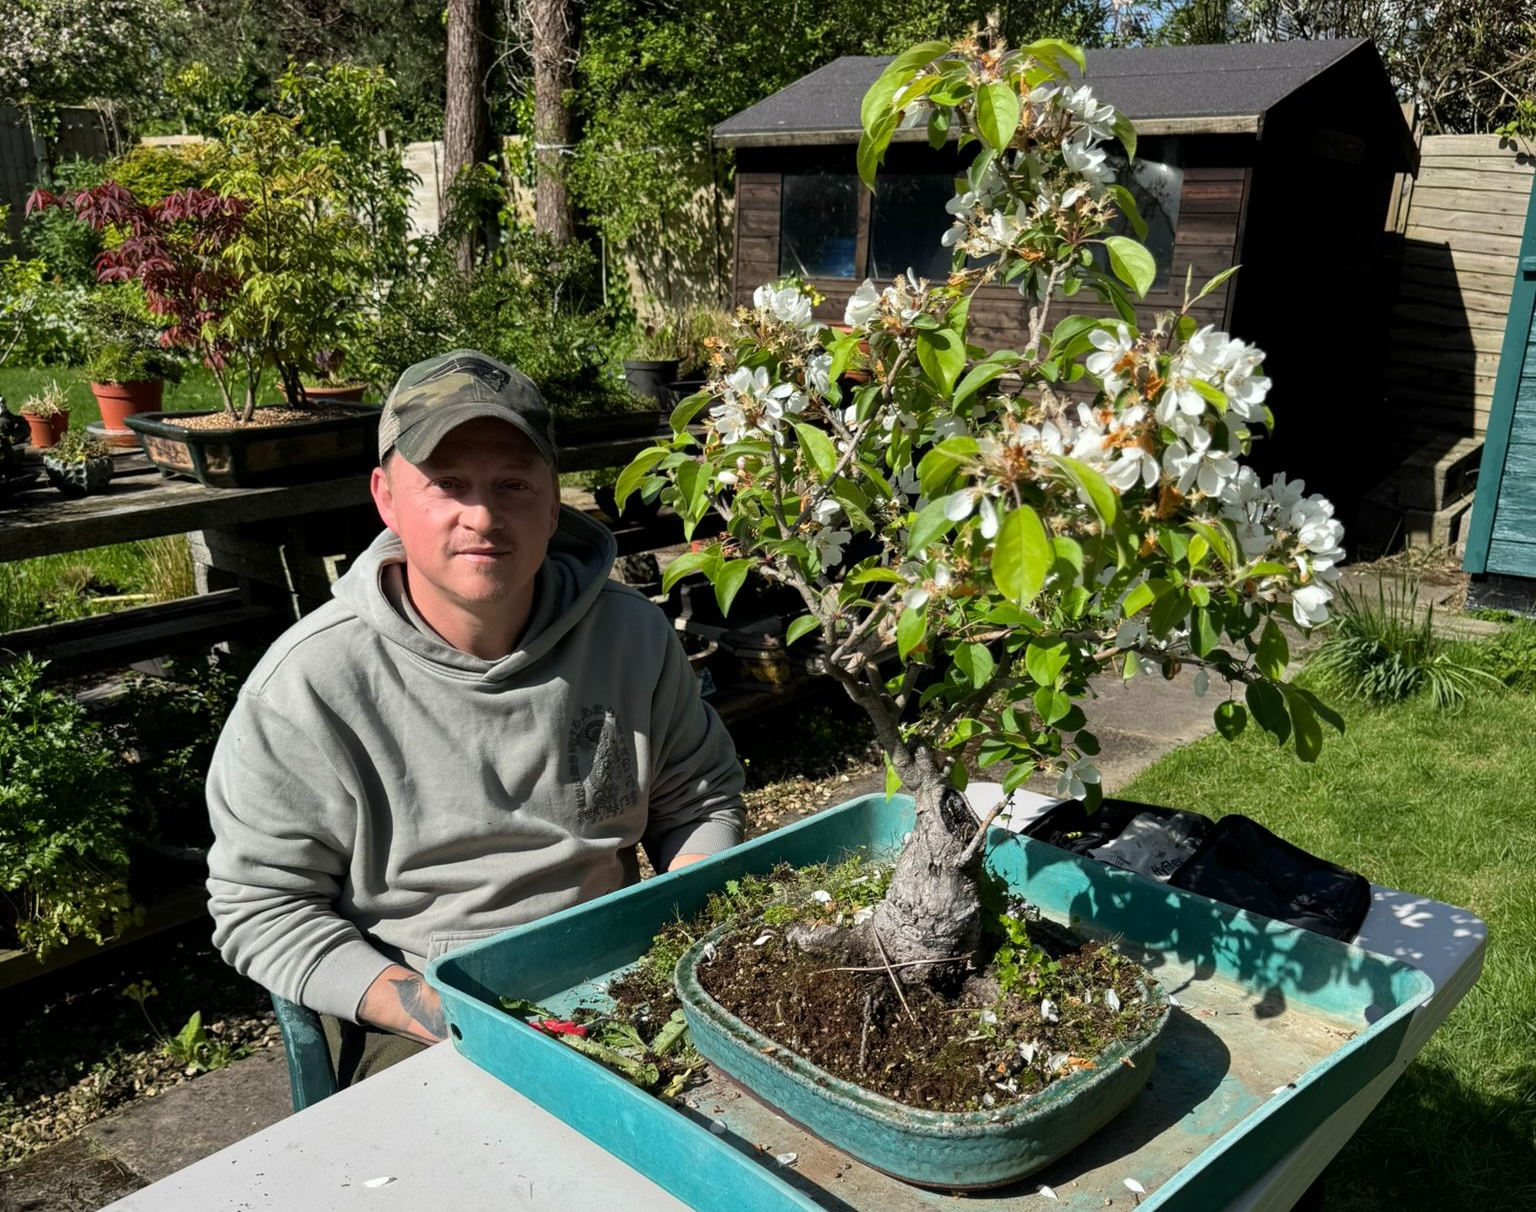
\includegraphics[width=1.0\columnwidth]{2025_05/res/gossip_david_barton_1},]
\end{window}
\vspace{-1em}
\begin{window}[2,l,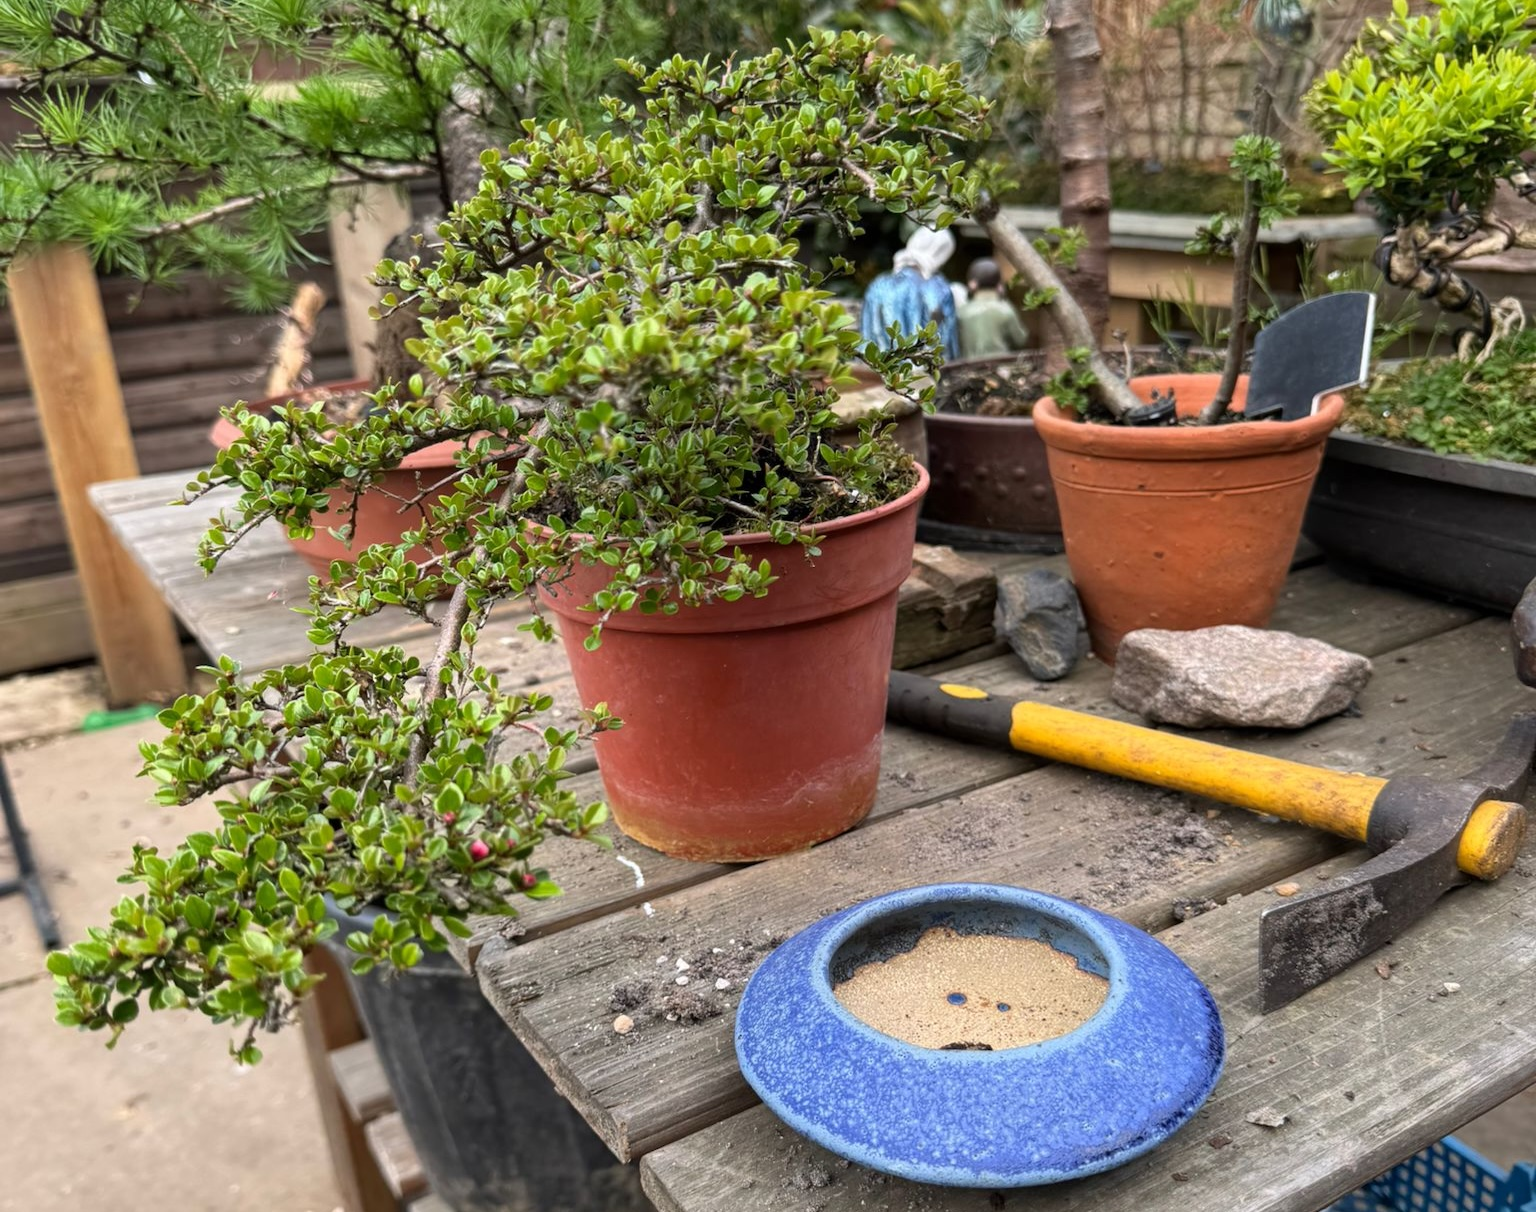
\includegraphics[width=1.0\columnwidth]{2025_05/res/gossip_david_barton_2},\centerline{\emph{David working on one of Dan Barton's trees.}}]
\end{window}

\columnbreak

Dan generously shared his wisdom and even his materials. \textit{``I wasn't expecting it,''} David says, \textit{``but I came away with a cotoneaster and a `flying saucer' pot---one of only a few Dan has made this year.''} A rare memento indeed, from a meaningful visit.

Opportunities like this remind us of the strength of our community---where passion, mentorship, and kindness often go hand in hand. We wish David the very best as he brings all he's learned to the competition bench.

\closearticle


\headline{{\textbf{\Large\sffamily Potting Shed Gossip:}}\\
{\textbf{\large\sffamily A Master's Tip in a Mouldy Box}}}
% \label{2025-05-gossip}
\noindent
This month, \textbf{Chris Durne} brought the past back to life. While patching up his garage's roof (between dodging spiders and shifting old boxes), he uncovered a stack of issues of the \textit{British Bonsai Association Bulletin}---bonsai history in paper form!

Chris, who's been delving into the early days of UK bonsai clubs, struck gold. Among the yellowing pages were quotes from none other than \textbf{John Naka}, the legendary American bonsai master behind masterpieces like \textit{Goshin}. We all know the classic, \textit{``There is no such thing as a finished bonsai.''} But another gem stood out:

\vspace{-1em}
% \medskip
\begin{quote}
\textit{\textbf{``To style the top of a tree, treat it as a separate bonsai and you will not go wrong.''}}
\end{quote}
% \medskip
\vspace{-1em}

Deceptively simple, quietly brilliant: it all makes sense.
% Next time you're wrestling with the apex, just imagine you're styling a whole new tree up there. 
% Suddenly, it all makes sense.

\noindent
\textit{Got a bonsai\--related rumour, quirky story, or fun fact?}
\noindent
\textit{Share it with us for the next edition of \textit{Potting Shed Gossip!}}

\begin{window}[2,l,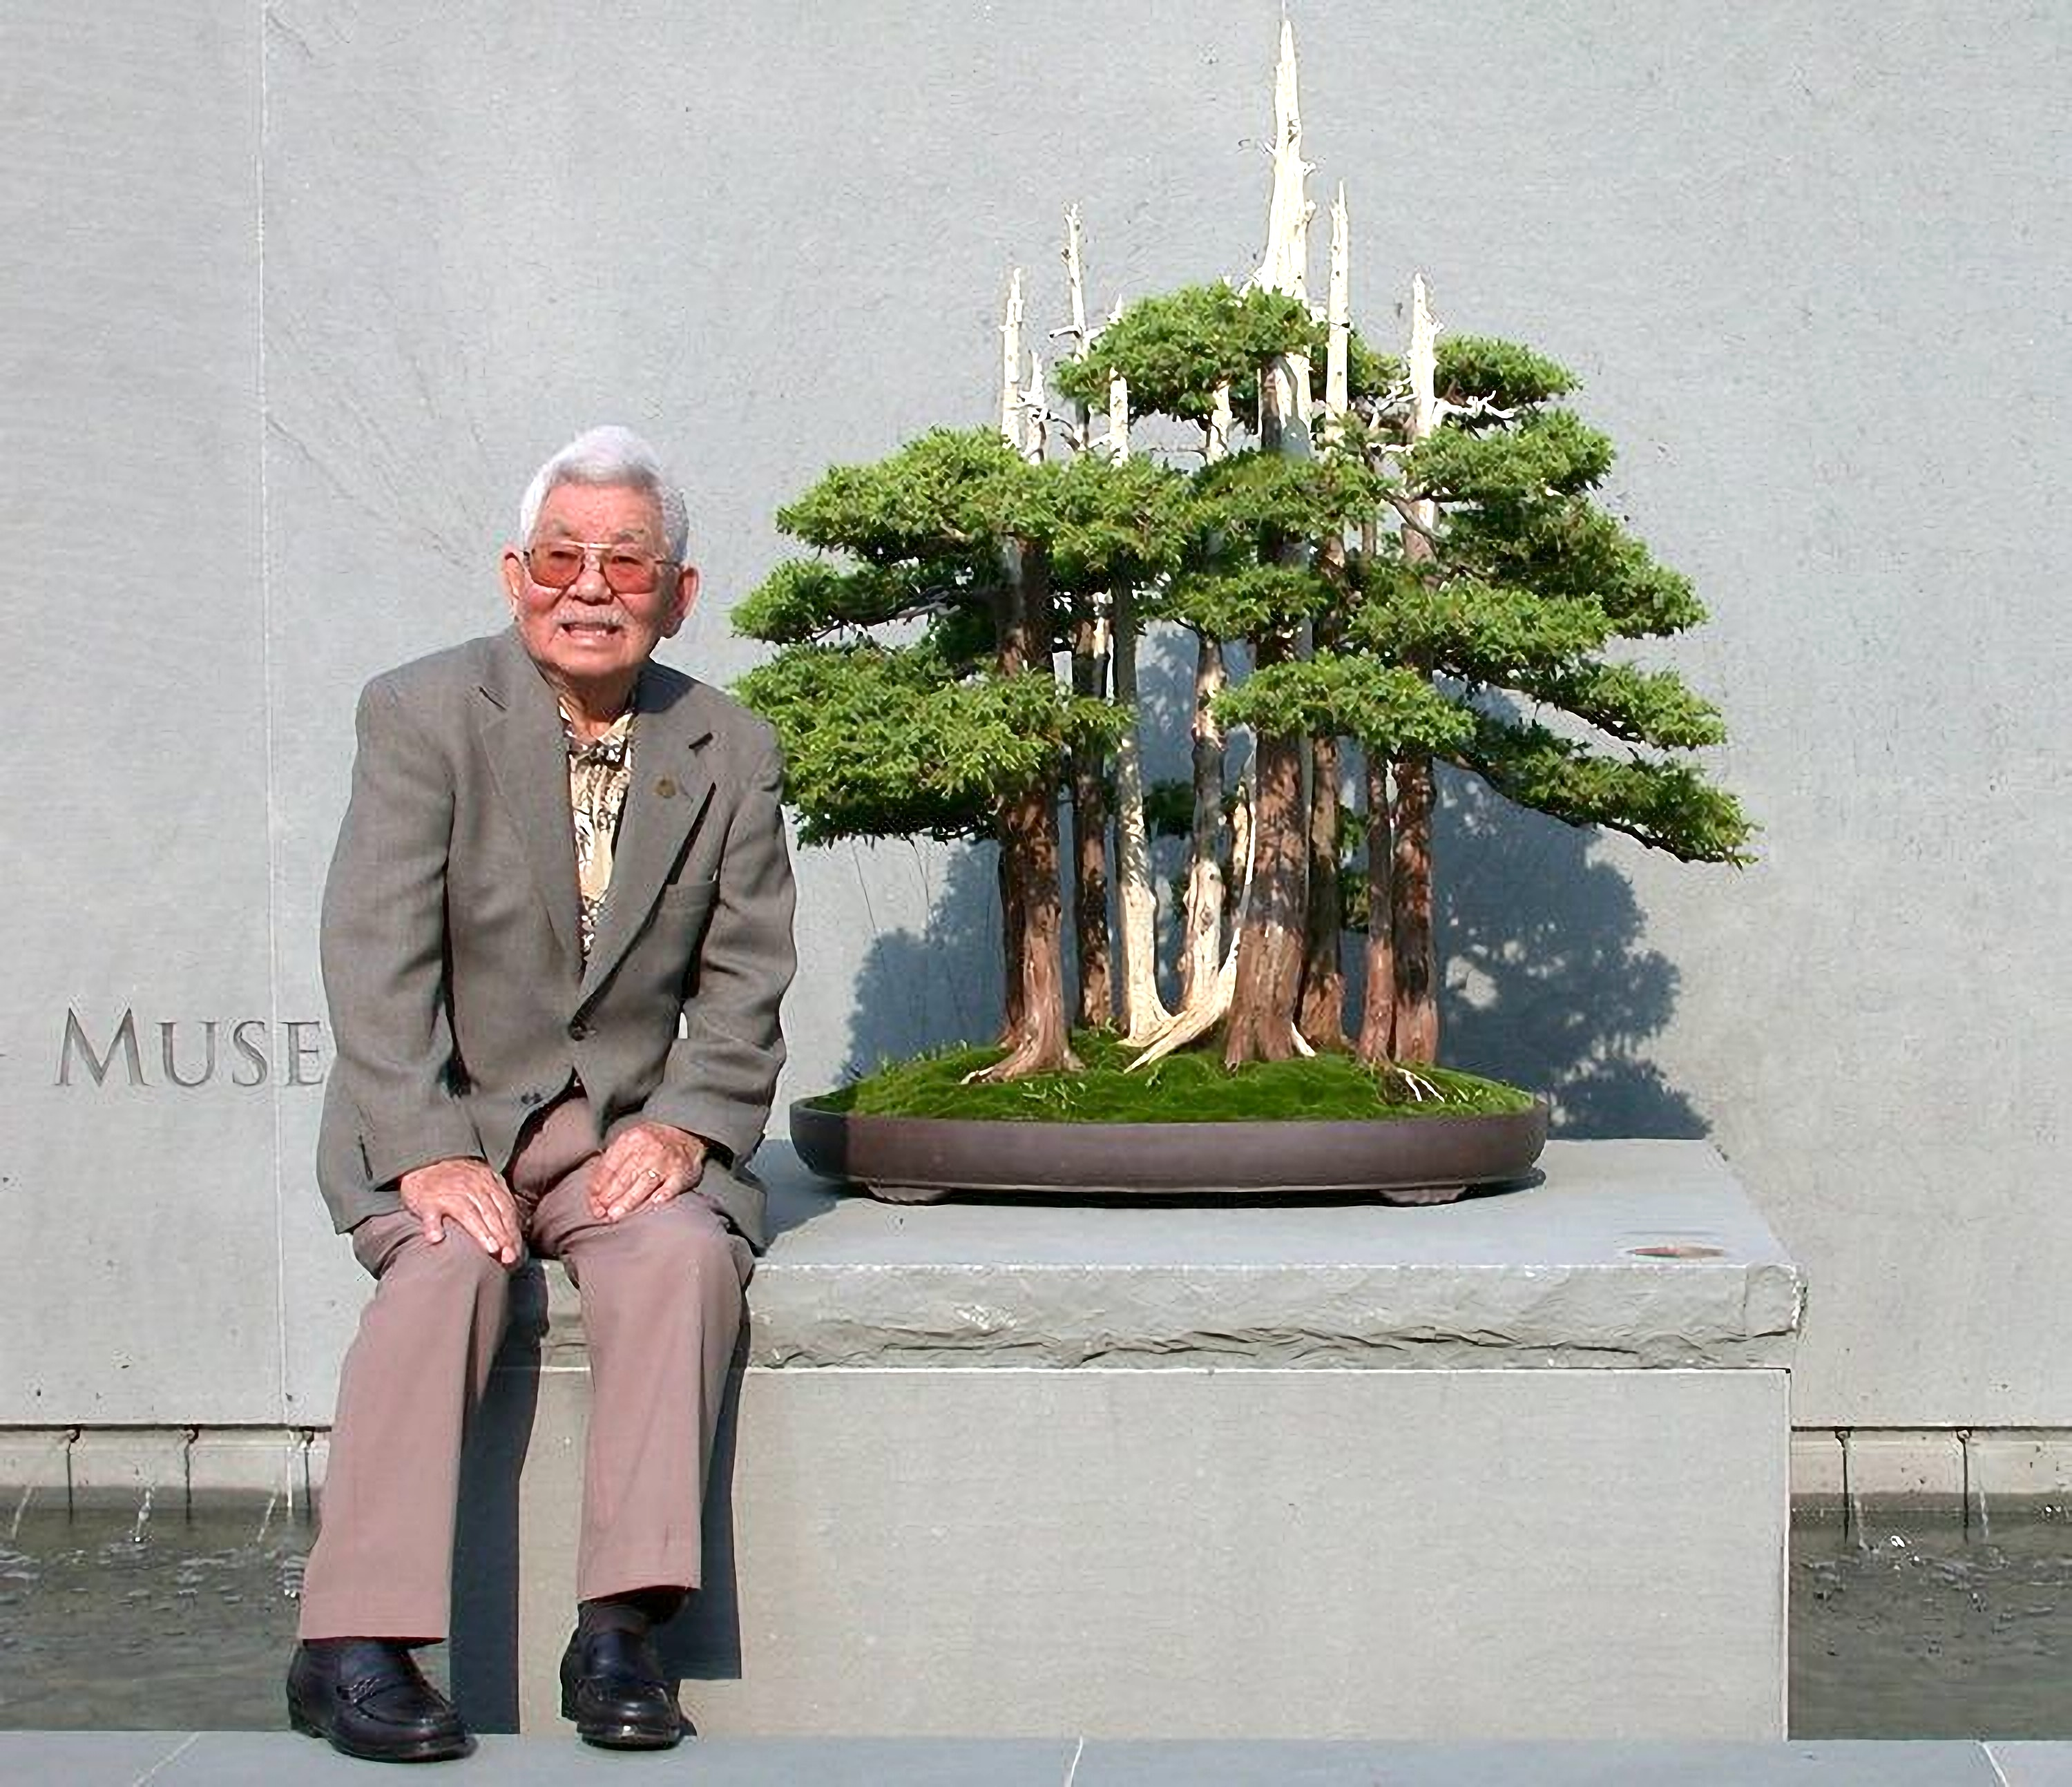
\includegraphics[width=1.0\columnwidth]{2025_05/res/gossip_naka_goshin},\centerline{\emph{John Naka and Goshin (courtesy of Wikipedia).}}]
\end{window}

\closearticle

\columnbreak
